\section{Discussion}

The Class Buffer model is more scalable over the three facets compared to other frameworks for viewing large scale data: data size, perceptual processing, and computation speed.
The enhanced perceptual processing arises from the broad spectrum of visualization methods that can be generated for density maps of multiple classes.
The model on the other hand does not guide users in a very good way. The challenges of understanding and using the different visualization methods have to be further investigated.
Multiclass density maps often have the disadvantage of obfuscating information when mixing or masking is introduced but they can also display more data classes that can be easily shown when using dot density maps. Different classes intersect, overlap and interfere with each other and by this make it hard to understand these kind of maps.
There are a multitude of visualization results that appear to visualize the data in a reasonably good way, but often the results obfuscate the data in a way that makes it hard to comprehend the full scope of the information present. In example the data that gets presented often mix or mask certain areas of interest. This results in clusters being mixed with neighboring clusters and thus losing the possibility to show the true amount of datapoints present in one group. Additionally outliers get overlaid by datapoints from other groups or get scaled down to an extend that they cannot be perceived at all when using the visualization methods provided by the Class Buffer model implementation, this effect can be seen in Figure~\ref{fig:outliers}.

\begin{figure}
	\centering
	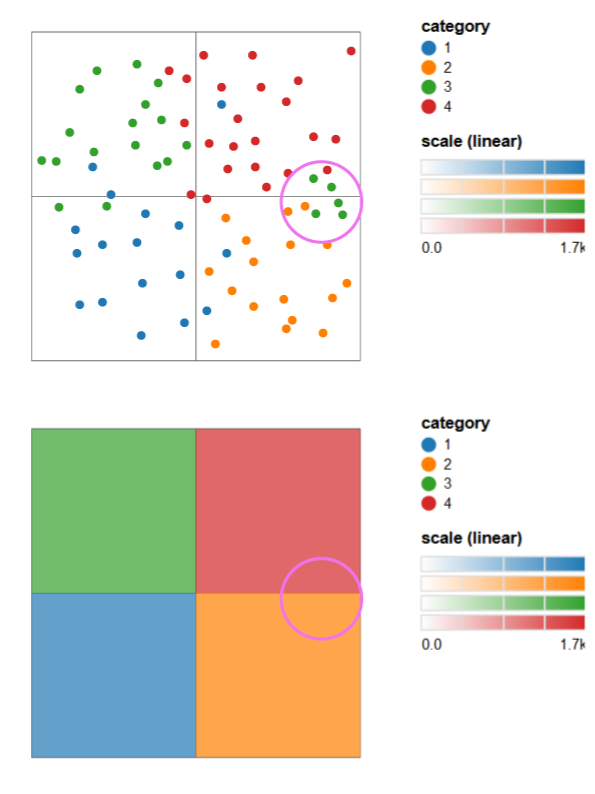
\includegraphics[width=0.85\columnwidth]{./figures/outliers}
	\caption[outliers]{A portrayal of the effect present when masking classes with other classes. In the top picture the data is visualized as a standard 2D scatterplot. The group of outliers get lost in the visualization process, which can be seen in the bottom picture.}~\label{fig:outliers}
\end{figure}

The Class Buffer model implemented by Jo et al. uses different approaches to display data but just few of them result in classical density maps~\cite{jo2019declarative}, some also arouse the impression of dot density maps with different tiling or aggregation.
A density map can be more challenging to comprehend when used in the wrong context or when implemented wrong or without an appropriate understanding of the field.\\It is thus essential to improve the presented method further. This could be done by enhancing the visual separation with additional options or by implementing an expressive guiding toolbox or some other kind of guideline. By providing the user with the basic tools to generate multiclass density maps the first step has been taken.

% \textcolor{red}{\lipsum[1]}

% \improvement{Clusters are seperable, outliers get lost}
